\chapter{Credit Risk}\label{credit_default_swaps}

Credit risk is the possibility of a loss resulting from a borrower's failure to repay a loan or meet contractual obligations. Traditionally, it refers to the risk that a lender may not receive the owed principal and interest, which results in an interruption of cash flows and increased costs for collection. 

Although it's impossible to know exactly who will default on obligations, properly assessing and managing credit risk can lessen the severity of a loss. Interest payments from the borrower or issuer of a debt obligation are a lender's or investor's reward for assuming credit risk.

In this Chapter the definition of credit event is introduced together with the Credit Default Swaps, a new type of instrument whose value depends on the likelihood that a given company will suffer a credit event over a given period.

\section{Credit curves}
\label{credit-curves}

A \textbf{credit event} can be a default, the failure to make payments, the issuer entering into bankruptcy proceedings, or the occurrence of other legal events. The exact definition of what constitutes a credit event depends on a series of factors and is usually defined in some kind of ISDA (International Swaps and Derivatives Association) master agreement. In any case, we will generically call with credit event a \emph{default}.

\textbf{Non-default probability} (NDP or survival probability) is the probability that a company will not suffer a credit event \textbf{before} a given date (i.e. non-default probability is a cumulative probability).

\textbf{credit curves} are a way of representing survival probabilities, and just like discount curves, they are built by specifying a sequence of pillar dates to which corresponds a sequence of NDPs. 

%Just like a discount curve is a way of representing the underlying interest rates implicit in the market quotes of a collection of interest rate products, implied by credit default swaps, a new kind of contract that will be introduced later.

\subsection{Hazard Rate or Default Intensity}
\label{hazard-rate}

The \textbf{hazard rate} represents the instantaneous probability of a party defaulting conditioned on it not having defaulted until that moment. Indeed it is often called a \emph{conditional failure rate} since its expression is a direct application of the conditional probability concept.

%It is related to credit curve like the short rate is to discount curves (the short rate, $r_t$, is the interest rate at which an entity can borrow money for an infinitesimally short period of time from time $t$). 

\subsubsection{Conditional Probability}
Conditional probability answers to the question "how should you update the probability of an event when there is additional information available ?". To derive the general formula let's start with an example.

A fair die is rolled. Let $A$ be the event set that the outcome is an odd number ($A={1,3,5}$). Also let $B$ be the event set that the outcome is less than or equal to $3$ ($B={1,2,3}$). What is the probability of $A$ ($P(A)$) ? And what is the probability of $A$ given $B$, the probability we get $A$ conditioned to having also $B$ ($P(A|B)$) ?

Being a simple example we can compute the result by hand:

\begin{equation}
P(A) = \cfrac{|A|}{|S|} = \cfrac{|\{1,3,5\}|}{6} = \cfrac{1}{2}\qquad\textrm{(where S is the entire sample space)}
\end{equation}

Now let's find the conditional probability of $A$ given that $B$ occurred. If we know $B$ has occurred, the outcome must be among $\{1,2,3\}$. For $A$ to also happen the outcome must be in $A\cap B = \{1,3\}$. Since all die rolls are equally likely, we argue that $P(A|B)$ must be equal to

\begin{equation}
P(A|B) = \cfrac{|A\cap B|}{|B|} = \cfrac{2}{3}
\end{equation}

To generalize our example we can rewrite the calculation by dividing the numerator and denominator by the entire space of the events $|S|$ hence:

\begin{equation}
P(A|B) = \cfrac{|A\cap B|}{|B|} = \cfrac{\cfrac{|A\cap B|}{|S|}}{\cfrac{|B|}{|S|}} = \cfrac{P(A\cap B)}{P(B)}
\end{equation}
See Figure~\ref{fig:conditional_prob} for a graphical interpretation of conditional probability.

\begin{figure}[tb]
\centering
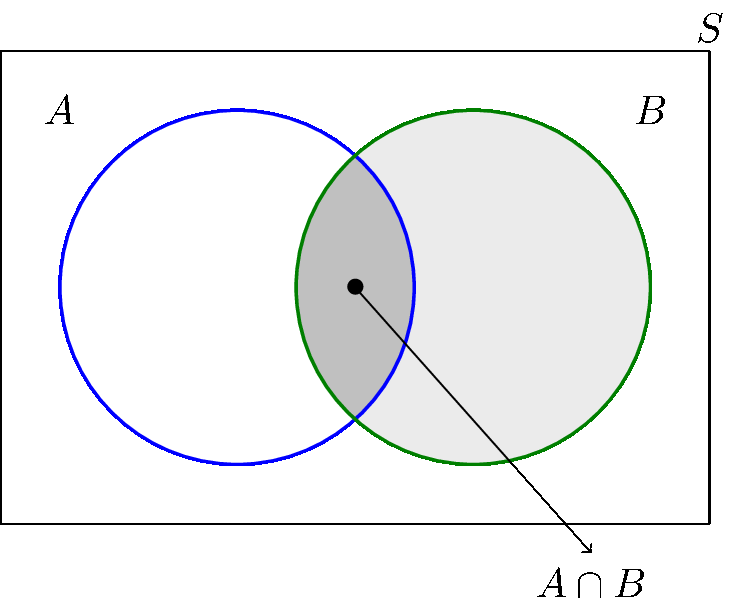
\includegraphics[width=0.5\linewidth]{figures/conditional_b}
\caption{Graphical representation of conditional probability (the gray shaded area).}
\label{fig:conditional_prob}
\end{figure}
.
\subsubsection{Hazard Rate Definition}
We can now compute the instantaneous default probability conditional to no previous default ($\lambda$), the \emph{hazard rate}~\cite{bib:hazard}.

%\[\lambda(t) = \cfrac{\mathbb{P}(A\cap B)}{\mathbb{P}(B)} = \cfrac{\cfrac{DP(\tau\in (t, t+dt))}{dt}}{DP(\tau>t)} = \cfrac{\cfrac{d[1-N(t_0, t)]}{dt}}{N(t_0, t)} = -\cfrac{dN(t_0, t)}{dt}\cdot\frac{1}{N(t_0, t)}\]
\begin{equation}
\begin{split}
\lambda(t)& = \lim_{dt\rightarrow 0} \cfrac{P_{\textrm{def}}(t, t+dt|\tau> t)}{dt} = \cfrac{dP_{\textrm{def}}(t)}{P_{\textrm{def}}(t, +\infty)}\cfrac{1}{dt}\\[5 pt] &
= \cfrac{d(1-P_{\textrm{sur}}(t_0 t))}{P_{\textrm{sur}}(t_0, t)}\cfrac{1}{dt} = -\cfrac{dP_{\textrm{sur}}(t)}{dt}\cfrac{1}{P_{\textrm{sur}}(t_0, t)}
\end{split}
\end{equation}
where $P_{\textrm{sur}}$ and $P_{\textrm{def}}$ are survival and default probabilities and $\tau$ the occurrence time of the credit event.
Also remember that $P_{\textrm{def}}(t_0, t) = 1 - P_{\textrm{sur}}(t_0, t)$. Given the hazard rate, the survival probability can be determined as:

%So far we have assumed implicitly that the credit event is bound to occur, so that $dP_{\textrm{sur}}(+\infty)=0$. Given enough time the survival probability goes down to zero. This condition implies that the cumulative hazard must diverge, i.e. we must have Λ(∞)=∞. Intuitively, the event will occur with certainty only if the cumulative risk over a long period is sufficiently high.

\begin{equation}
\begin{gathered}
\lambda(t) = -\cfrac{1}{dt}\cdot\cfrac{dP_{\textrm{sur}}(t_0, t)}{P_{\textrm{sur}}(t_0, t)} = -\cfrac{d(\textrm{log}P_{\textrm{sur}}(t_0, t))}{dt} \implies d(\textrm{log}P_{\textrm{sur}}(t_0, t)) = -\lambda dt\\[5pt]
P_{\textrm{sur}}(t_0, t) = \mathrm{exp}\left(-\int_{t_0}^{t}\lambda(s) ds\right)
\end{gathered}
\end{equation}

In practice hazard rate will be calculated numerically, and therefore we will consider the \emph{annualized} conditional probability of the issuer defaulting between a date and the next.

\label{sec:constant_hazard_rate}
The simplest possible survival distribution is obtained by assuming a constant risk over time, so the hazard is $\lambda (t)=\lambda$ for all $t$. The corresponding survival function is $P_{\textrm{sur}}(t_0, t) = e^{−\lambda (t-t_0)}$.

\subsection{Poisson Process}
\label{sec:poisson_process}
This kind of default (or survival) distributions belongs to a class of models called \emph{Poisson processes}. 
They can be used to model the frequency of events during a certain period of time assuming that one knows the average occurrence of those events over some period of time. 
Their general form is

\begin{equation}
P_X(k) = \frac{e^{-\lambda} \lambda)^{k}}{k!}
\label{eq:poisson_distribution}
\end{equation}

The Poisson process has a remarkable substructure. Even though the number of occurrence of events is modeled using a \emph{discrete} Poisson distribution, Eq.~\ref{eq:poisson_distribution}, the interval of time between consecutive events can be modeled using an exponential distribution, which is a \emph{continuous} distribution.

The probability density function of the random variable describing the time to the next event is:

\begin{equation}
P_X(t) = \lambda e^{-\lambda t}
\label{eq:inter-arrival}
\end{equation}
and its cumulative distribution function is:

\begin{equation}
F_X(t) = P(X<=t) = \int_{0}^{t}\lambda e^{-\lambda x} dx = 1 - e^{-\lambda t}
\label{eq:inter-arrival}
\end{equation}

which is the same function obtained for the default probability in case of constant hazard rate, see~\ref{sec:constant_hazard_rate}.
Recollect that CDF of $X$ returns the probability that the interval of time between consecutive events will be less than or equal to some value $t$.
Finally the inverse function of the CDF is:
\begin{equation}
F^{-1}(X) = -\frac{\log(1-X)}{\lambda}
\end{equation}

\begin{finmarkets}
We now have enough information to simulate events (i.e. defaults) according to Poisson process. 

The following class is an \emph{extension} of \texttt{scipy.stats} that implements distributions of the form $\lambda e^{-\lambda t}$. This is another example of \emph{sub-classing} an existing class (inheritance, see Section~\ref{inheritance-and-overriding-methods}) since its parent is \texttt{rv\_continuous} the starting point for each continuous distribution in \texttt{scipy}.

Once the default intensity has been set, we can model the cumulative default probability over a certain period of time using the \texttt{cdf} method. Contrary feeding different probability values, using the inverse-CDF (the \texttt{ppf} method), gives us the corresponding default times for the respective probabilities.
\end{finmarkets}

\begin{ipython}
from scipy.stats import rv_continuous
import numpy as np
	
class ExpDefault(rv_continuous):
    def __init__(self, l):
        super().__init__()
        self.l = l
	
    def _cdf(self, x):
        x[x < 0] = 0
        return (1 - np.exp(-self.l*x))
	
    def _pdf(self, x):
        x[x < 0] = 0
        return self.l*np.exp(-self.l*x)
	
    def _ppf(self, x):
        return -np.log(1-x)/self.l
\end{ipython}


\begin{finmarkets}
Similarly to discount curves we implement a class to handle credit curves, \texttt{CreditCurve}. It is characterized by a list of pillar dates with the corresponding survival probabilities. Like the \texttt{DiscountCurve} object you don't need to pass the curve today's values (survivial probability 1) since it is done automatically by the class constructor. Two methods are available: one to interpolate survival probabilities and the second to compute the hazard rate at any arbitrary date (beware that extrapolation is not allowed so the input date must be within the pillar dates range).
\end{finmarkets}

\begin{ipython}
from numpy import interp
from dateutil.relativedelta import relativedelta
	
class CreditCurve:
    def __init__(self, obs_date, pillar_dates, ndps):
        self.obs_date = obs_date
        self.pillar_dates = [obs_date] + pillar_dates
        self.pillar_days = [(pd - obs_date).days for pd in self.pillar_dates]
        self.ndps = np.insert(np.array(ndps), 0, 1)
	
    def ndp(self, d):
        d_days = (d - self.obs_date).days
        if d < self.obs_date or d_days > self.pillar_days[-1]:
            print ("Cannot extrapolate survival probabilities (date: {}).".format(d))
            return None
        return np.interp(d_days, self.pillar_days, self.ndps)
	
    def hazard(self, d):
        ndp_1 = self.ndp(d)
        ndp_2 = self.ndp(d + relativedelta(days=1))
        delta_t = 1.0 / 365.0
        h = -1.0 / ndp_1 * (ndp_2 - ndp_1) / delta_t
        return h
\end{ipython}

Let's test the class with some inputs.
\begin{ipython}
from datetime import date
from dateutil.relativedelta import relativedelta
	
obs_date = date.today()
cc = CreditCurve(obs_date, [obs_date + relativedelta(years=2)], [0.8])
	
print (cc.ndp(obs_date + relativedelta(years=1)))
\end{ipython}
\begin{ioutput}
0.9001367989056088
\end{ioutput}
\begin{ipython}
print(cc.hazard(obs_date + relativedelta(years=1)))
\end{ipython}
\begin{ioutput}
0.11094224924016097
\end{ioutput}

\section{Credit Default Swaps}
\label{sec:credit-default-swaps}

%Once we have implemented a \texttt{CreditCurve} class which allows to interpolate survival probabilities and also to calculate the hazard rate at arbitrary dates, we can use it to price \textbf{Credit Default Swaps} (CDSs).

A Credit Default Swap (CDS) is a financial agreement in which the seller commit to compensate the buyer in case of a default or other credit event. That is, the seller of the CDS "insures" the buyer against some reference asset defaulting. In exchange the buyer of the CDS makes a series of payments (the CDS \emph{spread}) to the seller.

\subsection{Valuation of CDS}
\label{sec:cds_valuation}

Credit Default Swaps are made up of two legs:

\begin{itemize}
\tightlist
\item the \emph{premium} leg: which pays the spread $S$ periodically until a credit event occurs;
\item the \emph{default} leg: which pays $L = F(1 - R)$, known as the \textbf{loss given default} (LGD), if and when the credit event occurs ($F$ is the notional of the contract, $R$ is the \textbf{recovery rate} or the percentage of the loss recovered from a default. The recovery rate varies by industry, the degree of seniority in the capital structure, the amount of leverage in the capital structure in total, and whether a particular security is secured or otherwise collateralized. A common baseline assumption is to set it to 40\%.
\end{itemize}

\subsubsection{Premium leg}\label{premium-leg}

In the valuation of the premium leg, we'll use the following notation:

\begin{itemize}
\tightlist
\item $d$ pricing date;
\item $d_0$ the start date of the CDS (could be different from pricing date);
\item $d_1, ..., d_n$ the payment dates of the premium leg. We assume that $d_n$ is the end date of the CDS;
\item $D(d')$ the discount factor between $d$ and $d'$;
\item $P_{\textrm{sur}}(d, d')$ the survival probability between $d$ and $d'$;
\item $\tau$ the \emph{random variable} representing the credit event date.
\end{itemize}

At each payment date $d_i$, a cash flow of $F\cdot S$ is paid if and only if the credit event has \emph{not} occurred before that date. Therefore the NPV of each flow is

\begin{equation}
f_{\textrm{premium}}^i = \mathbb{E}\left[F\times S \times D(d_i) \times \mathbb{1}(\tau > d_i) \right]
\end{equation}
where the indicator function $\mathbb{1}(\tau > d_i)$ means that the expectation value has to be evaluated when $\tau > d_i$. 

Since the NPV depends on the random variable $\tau$, the estimate of its value needs to be done through an expectation.
Remembering the definition of expected value (see Section~\ref{sec:expected-value}), %we can interpret 
%\(F\cdot S\cdot D(d_i)\) as the variables and $P_{\textrm{sur}}(d, d_i)$ as the probabilities so 
the premium leg NPV can be expressed as:

\begin{equation}
\textrm{NPV}_{premium} = F\cdot S \cdot \sum_{i=1}^{n} D(d_i) \cdot P_{\textrm{sur}}(d, d_i)
\end{equation}

\subsubsection{Default leg}
\label{default-leg}

We assume that as soon as a credit event occurs (at a time $\tau$) the LGD is paid out (i.e. on the same date, but could potentially be paid on any date between $d_0$ and $d_n$). Mathematically, therefore, the NPV of the default leg can be expressed as follows:

\begin{equation}
\mathrm{NPV_{default}} =\mathbb{E}[F(1-R) \times D(\tau) \times \mathbb{1} \{\tau \leq d_n\} ]
\end{equation}

Also in this case we are dealing with a probabilistic event so the expectation value has to be computed taking into account the payments $F(1-R)\times D(\tau)$ averaged over the default probability $P_{\textrm{def}}(d, \tau)$. 

Using the law of total probability, we can break the previous expression down into the sum of "daily NPVs" calculated as a function of the \emph{daily} default probabilities:

\begin{align}
\begin{split}
\mathrm{NPV_{default}} &= \mathbb{E}[F(1-R) \times D(\tau) \times \mathbb{1}\{\tau \leq d_n\} ] \\
&= \sum_{d'=d_0}^{d_n} F(1-R) \cdot D(\tau = d') P_{\textrm{def}}(d, \tau = d') \\
&= F(1-R) \sum_{d'=d_0}^{d_n} D(d') \left(P_{\textrm{def}}(\tau \geq d') - P_{\textrm{def}}( \tau \geq d'+1) \right) \\
&= F(1-R) \sum_{d'=d_0}^{d_n} D(d') \left( P_{\textrm{sur}}(d, d') - P_{\textrm{sur}}(d, d'+1) \right)
\end{split}
\end{align}
where the last step holds since $P_{\textrm{def}}(\tau\geq d') = 1 - P_{\textrm{def}}(\tau < d') = 1 - (1-P_{\textrm{sur}}(d, d')) = P_{\textrm{sur}}(d, d')$. 
Figure~\ref{fig:default_p} illustrates the steps to convert the daily default probability $P_{\textrm{def}}(d, \tau=d')$.

\begin{figure}[htb]
\centering
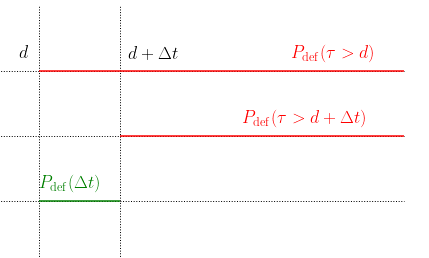
\includegraphics[width=0.7\textwidth]{figures/timeline.png}
\caption{The probability that a default occurs at a time $\tau = d+\Delta t$ is equivalent to the default probability at $\tau > d$ minus the default probability at $\tau>d+\Delta t$.}
\label{fig:default_p}
\end{figure}

\begin{finmarkets}
As for the other kind of contracts we develop also a \texttt{CreditDefaultSwap} class. In this case the class has methods to compute NPVs for the premium and default legs. 

The break-even spread of a credit default swap is the value of the fixed rate paid in the premium leg that makes the CDS net present value equal to 0.

To determine the break-even spread is enough to impose that the NPV of the premium and default legs are equal:

\begin{equation}
S \cdot\sum_{i=1}^{n} D(d_i) \cdot P_{\textrm{sur}}(d, d_i)
= (1-R) \sum_{d'=d_0}^{d_n} D(d') \left( P_{\textrm{sur}}(d, d') - P_{\textrm{sur}}(d, d'+1) \right)
\end{equation}
solving for $S$ we obtain the wanted spread

\begin{equation}
S_{\mathrm{breakeven}} = \cfrac{(1-R) \sum_{d'=d_0}^{d_n} D(d') \left( P_{\textrm{sur}}(d, d') - P_{\textrm{sur}}(d, d'+1) \right)}{\sum_{i=1}^{n} D(d_i) \cdot P_{\textrm{sur}}(d, d_i)}
\end{equation}
\end{finmarkets}

\begin{ipython}
from finmarkets import generate_dates

class CreditDefaultSwap:
    def __init__(self, nominal, start_date, maturity, fixed_spread,
                 tenor="3m", recovery=0.4):
        self.nominal = nominal
        self.payment_dates = generate_dates(start_date, maturity, tenor)
        self.fixed_spread = fixed_spread
        self.recovery = recovery

    def npv_premium_leg(self, discount_curve, credit_curve):
        npv = 0
        for i in range(1, len(self.payment_dates)):
            npv += (discount_curve.df(self.payment_dates[i]) *
                    credit_curve.ndp(self.payment_dates[i]))
        return self.fixed_spread * npv * self.nominal

    def npv_default_leg(self, discount_curve, credit_curve):
        npv = 0
        d = self.payment_dates[0]
        while d < self.payment_dates[-1]:
            npv += discount_curve.df(d) * (
                   credit_curve.ndp(d) -
                   credit_curve.ndp(d + relativedelta(days=1)))
            d += relativedelta(days=1)
        return npv * self.nominal * (1 - self.recovery)

    def npv(self, discount_curve, credit_curve):
        return self.npv_default_leg(discount_curve, credit_curve) - \
               self.npv_premium_leg(discount_curve, credit_curve)
\end{ipython}

To test the class data contained in \href{https://github.com/matteosan1/finance_course/raw/master/input_files/discount_factors_2022-10-05.xlsx}{discount\_factors\_2022-10-05.xlsx} is used.

\begin{ipython}
import pandas as pd
from finmarkets import DiscountCurve
from dateutil.relativedelta import relativedelta
from datetime import date

dc_data = pd.read_excel("discount_factors_2022-10-05.xlsx")
obs_date = date.today() 
start_date = obs_date
dates = [obs_date + relativedelta(months=i) for i in dc_data['months']]
dc = DiscountCurve(obs_date, dates, dc_data['dfs'])

pillars = [obs_date + relativedelta(months=36)]
credit_curve = CreditCurve(obs_date, pillars, [0.7])
cds = CreditDefaultSwap(1e6, start_date, "3y", 0.03)

# check default leg, premium leg and npv
print ("Premium leg: {:.2f} EUR".format(cds.npv_premium_leg(dc, credit_curve)))
print ("Default leg: {:.2f} EUR".format(cds.npv_default_leg(dc, credit_curve)))
print ("NPV: {:.2f} EUR".format(cds.npv(dc, credit_curve)))
\end{ipython}
\begin{ioutput}
Premium leg: 303120.25 EUR
Default leg: 180903.50 EUR
NPV: -122216.74 EUR
\end{ioutput}
	
%\section{Credit Ratings}\label{credit-ratings}
%
%A credit rating is a quantified assessment of the creditworthiness of a borrower either in general terms or with respect to a particular debt or financial obligation. A credit rating can be assigned to any entity that seeks to borrow money (e.g. an individual, corporation, state or provincial authority, or sovereign government).
%
%A loan is a essentially a promise and the credit rating determines the likelihood that the borrower will be able to pay back it within the loan agreement terms. A high credit rating indicates a high possibility of paying back the loan in its entirety without any issue; a poor credit rating suggests that the borrower has had trouble paying back loans in the past and might follow the same pattern in the future.
%
%Individual credit is scored from credit bureaus (e.g. Experian and TransUnion) and it is reported as a number, generally ranging from 300 to 850.
%
%Credit assessment and evaluation for companies and governments instead is generally done by credit rating agencies (e.g. Standard \& Poor's (S\&P), Moody's, or Fitch), which typically assign letter grades to indicate ratings. Standard \& Poor's, for instance, has a credit rating scale ranging from AAA (excellent) to C and D. A debt instrument with a rating below BB is considered to be a speculative grade or a junk bond, which means it is more likely to default on loans.
%
%\subsection{Why Credit Ratings Are Important}\label{why-credit-ratings-are-important}
%
%A borrowing entity will strive to have the highest possible credit rating since it has a major impact on interest rates charged by lenders. Rating agencies, on the other hand, must take a balanced and objective view of the borrower's financial situation and capacity to repay the debt.
%
%A credit rating not only determines whether or not a borrower will be approved for a loan but also determines the interest rate at which the loan will need to be repaid. Since companies depend on loans for many expenses, being denied a loan could spell disaster, and in any case a high interest rate is much more difficult to pay back.
%Credit ratings also play a large role in a potential investor's determining whether or not to purchase bonds. A poor credit rating is a risky investment; it indicates a larger probability that the company will be unable to make its bond payments.
%
%It is important for a borrower to remain diligent in maintaining a high credit rating. Credit ratings are never static; in fact, they change all the time based on the newest data, and one negative debt will bring down even the best score. 
%Credit also takes time to build up. An entity with good credit but a short credit history is not seen as positively as another entity with the same quality of credit but a longer history. Debtors want to know a borrower can maintain good credit consistently over time.

\section{Determine Default Probabilities from Market Quotes}
In this Section we find out how to derive default probabilities implied by market quotes, checking how it can be done both from bonds and Credit Default Swaps.

\subsection{Implied Probability of Default from Coupon Bonds}
\label{default-probabilities-and-bond-prices}

The price of a bond issued by a party is directly linked to the credit rating of that party, since there is always an associated default risk (the borrower might not be able to repay fully or partially the amount of the taken loan). 

Bonds with low ratings, called junk bonds, are sold at lower prices (since riskier), while those with higher ratings, called investment-grade bonds, are sold at higher prices.

%\subsubsection{Crude Approximation}

The average default intensity can be approximated by considering the spread $s$ between the rates of a risky and a risk-free bond, and the recovery rate $R$.

The risk-free zero coupon bond value $e^{-(r+s)\cdot T}$ equals that of the risky bond which can be computed remembering the expression for the default probability as a function of the hazard rate when this is constant (see Example~\ref{sec:constant_hazard_rate})

\begin{equation}
e^{-(r+s)\cdot T} = 
\begin{cases}
R\;\;\textrm{with probability}\;1 - e^{-\lambda T} \\
1\;\;\textrm{with probability}\;e^{-\lambda T} \\
\end{cases} = 
(e^{-\lambda T} + R - R e^{-\lambda T})e^{-rT}
\end{equation}

If $\lambda$ is small we can use the Taylor expansion neglecting orders higher than the first $e^{x} = 1 + x$ (the discount factor can be simplified away from both sides)

\begin{equation}
\begin{gathered}
e^{-sT} = e^{-\lambda T} + R - R e^{-\lambda T} \\
1 - sT = 1 - \lambda T + R - R(1 - \lambda T) = 1 - \lambda T + R - R + R\lambda T\\
\end{gathered}
\end{equation}
Simplifying and changing signs we are left with
\begin{equation}
s = (1 - R)\cdot \lambda \implies \lambda = \frac{s}{1-R}
\end{equation}

Imagine for example a bond that yields 150 basis points more than a similar risk-free bond and assume an expected recovery rate of 40\%.

\begin{equation*}
\bar{\lambda} = \cfrac{0.015}{(1-0.4)} = 2.5\%
\end{equation*}

% \subsubsection{Better Approximation}

% To estimate the default probability with a higher precision is possible to calculate the expected loss in terms of the unconditional default probability $Q$. As before

% \begin{equation}
% Q = \cfrac{s}{\sum\mathrm{expected\_losses}}
% \end{equation}
% where $s$ is now the difference in price between the risky and the risk-free bonds.

% Consider a 5-year corporate bond which provides an annual 6\% coupon (paid semiannually), with an yield of 7\%. The yield of a similar risk-free bond is instead 5\%. Assume a recovery rate of 40\% and that defaults can happen only immediately before coupon payment dates at times 0.5, 1.5, 2.5, 3.5 and 4.5. 

% Let's determine the unconditional default probability $Q$ in \texttt{python}.

% \begin{ipython}
% from math import exp
% import numpy as np

% default_dates = [0.5, 1.5, 2.5, 3.5, 4.5]
% R = 0.4

% def bond_price(N, C, y, maturity, tenor):
%     val = 0
%     for i in np.arange(tenor, maturity+tenor, tenor):
%         val += N*C*tenor*exp(-y*i)
%     val += N*exp(-y*i)
%     return val

% def expected_loss(N, C, r, maturity, tenor):
%     loss = 0
%     for i in range(len(default_dates)):
%         val = 0
%         for t in np.arange(default_dates[i], maturity+tenor, tenor):
%             val += N*C*tenor*exp(-r*(t-default_dates[i]))
%         val += N * exp(-r*(t-default_dates[i]))
%         val = (val-N*R)*exp(-r*default_dates[i])
%         loss += val
%     return loss

% Pr = bond_price(100, 0.06, 0.07, 5, 0.5)
% Prf = bond_price(100, 0.06, 0.05, 5, 0.5)
% spread = abs(Pr - Prf)
% print ("{:.2f}%".format(spread / expected_loss(100, 0.06, 0.05, 5, 0.5)*100))
% \end{ipython}
% \begin{ioutput}
% 3.03%
% \end{ioutput}

% This algorithm can be generalized for example by defining $Q$ as a function of the hazard rate. By using several bonds with different maturities also it is possible to derive the term structure of the default probability with an approach similar to the bootstrap.

%Let's see with an example how the default probability can be determined from bond prices. Imagine to have a bond and let \(x\) represent the present value of its cash flow stream. To valuate the bond when a default probability is associated to the issuer it is necessary to take each possible value of $x$ (the value of the bond), multiply it by the corresponding default probability and sum the results.  In other words the value of the bond should equal the mathematical expectation (see Section~\ref{sec:expected-value}) of $x$.
%
%Consider a bond which pays $F$ at maturity and that the issuer of this bond has a default probability $P$ (the recovery is $R$). What will be the price of this bond ?
%
%\begin{equation}
%V_{bond} =
%\begin{cases}
%& D \cdot R \cdot F\quad\textrm{(in case of default of the issuer)}\\
%&D \cdot F\quad\textrm{(in case of no default)}\\
%\end{cases}\end{equation} 
%where \(D\) is the proper discount factor. Since we don't
%know if the issuer will default or not we can estimate the bond price as
%
%\begin{equation}
%V_{bond} = D \cdot R \cdot F \cdot DP ( \tau ) + D \cdot F \cdot ( 1 − DP ( \tau)) = D\cdot F \cdot ( 1 − ( 1 − R ) DP ( \tau ))
%\end{equation}
%\noindent
%where $\tau$ represent the maturity date of the bond.
%From the this equation is clear that the higher the default probability the lower the bond price. Conversely, given the market price of the bond ($V_{bond}$) we can estimate the issuer default probability.
%
%%The probability of a company default can be estimated directly from
%%the prices of its issued bonds. Imagine that the spread $s$
%%between a corporate bond over the risk-free rate should compensate for
%%the losses in case of default, so naively:
%%
%%\[\lambda = \frac{s}{1-R}\]
%%where $\lambda$ is the annualised hazard rate and $R$ the recovery rate.
%
%%In a more detailed way let $X$ represents the present value of a bond cash flow stream. When you
%%have a default probability then $X$ becomes a random variable with a range
%%of possible values. The way
%%to value the bond in this case is to take each possible value of $X$, multiply it
%%by its probability and sum the results. In other words the value of the bond
%%should equal the mathematical expectation of $X$.
%
%\begin{attention}
%To generalize, consider the case of a bond with $N$ coupon payments until maturity. Let $S$ be the probability that the bond \emph{survives} from one coupon payment to the next and let $X_i$ ($i$ = 0, 1,\ldots, $N$) be the value of $X$ given that the bond defaults after making its $i$-th coupon payment. The expectation of $X$ can then be expressed as:
%
%\begin{align}
%\begin{split}
%\mathbb{E}(X) &= X_0(1-S) + X_1 S(1-S) + X_2 S^2 (1-S) + X_3 S^3 (1-S) + X_4 S^4 + \ldots \\
%&= X_0 + (X_1 - X_0)S + (X_2 - X_1)S^2 + (X_3 - X_2)S^3 + (X_4 - X_3)S^4 + \ldots
%\end{split}
%\end{align}
%
%Assuming a constant recovery value $R$ the values $X_i$ are:
%
%\begin{align}
%\begin{split}
%X_0 &= RF \\
%X_1 &= (C + RF)\cdot D \\
%X_2 &= C\cdot D + (C + RF)\cdot D^2 \\
%X_3 &= C\cdot D + C\cdot D^2 + (C + RF)\cdot D^3 \\
%X_4 &= C\cdot D + C\cdot D^2 + C\cdot D^3 + (C + F)\cdot D^4 \\
%\cdots 
%\end{split}
%\end{align}
%where $D$ represent the proper discount factor and $F$ the bond face value.
%Substituting into the expectation formula:
%
%\begin{align}
%\begin{split}
%\mathbb{E}(X) &= C((SD) + (SD)^2 + (SD)^3 + (SD)^4) + \\
%&RF(1-S)(1+(SD)+(SD)^2 + (SD)^3) + F(SD)^4 + \ldots
%\end{split}
%\end{align}
%
%It is now easy to write previous equation in a more compact form:
%
%\begin{equation} 
%\mathbb{E}(X) = C \sum_{k=1}^{N}{(SD)^k} + RF(1-S)\sum_{k=1}^{N-1}{(SD)^k} + F(SD)^N 
%\end{equation}
%
%Each of the sums in this s formula is a geometric series that can be collapsed into a single term. The formula for collapsing a general geometric series is 
%
%\begin{equation}
%\sum_{k=0}^N a^k = 1 + a + a^2 + \ldots + a^N = \cfrac{1-a^{N+1}}{1-a} 
%\end{equation}
%Hence we get:
%
%\begin{align}
%\begin{split}
%\mathbb{E}(X) &= (CSD) \cfrac{1-(SD)^N}{1-(SD)}+RF(1-S)\cfrac{1-(SD)^N}{1-(SD)} + F(SD)^N \\
%&= \Big(CSD + RF(1-S)\Big)\cfrac{1-(SD)^N}{1-(SD)} + F(SD)^N 
%\end{split}
%\end{align}
%
%With $\mathbb{E}(X)$ equal to the price of the bond, this equation can be solved numerically for the survival probability $S$.
%
%To get the default probability for the bond, simply subtract the survival probability from 1. The cumulative default probability, or the probability that the bond defaults anytime within the next $k$ coupon periods is $(1 - S^k)$.
%
%There are several ways to test the formula for logical consistency. First look at the case where the survival probability is zero so that with $S = 0$ the formula reduces to:
%
%\begin{equation}
%\mathbb{E}(X) = RF
%\end{equation}
%this is logical since when default is immanent the price should just equal the recovery amount. In the case where survival is certain and the risk free rate is zero you have $S = 1$ and $D=1$:
%
%\begin{equation}
%\mathbb{E}(X) = NC + F 
%\end{equation}
%The price here is equal to the total of the coupon payments plus the face value, as you would expect.
%
%Next an example with a \texttt{python} implementation which uses \texttt{brentq}.
%
%\begin{attpython}
%from scipy.optimize import brentq
%
%C = 0.05 # coupon
%r = 0.03 # risk-free rate
%D = 1/(1+r) # discount factor
%F=100 # bond face value
%R=0.4 # recovery
%N=4 # maturity
%trading_price = 80
%
%def func(x):
%    return C*x*D + R*F*(1-x)*(1-(x*D)**N)/(1-x*D)+F*(x*D)**N
%        -trading_price
%res = brentq(func, 0, 1)
%
%print ("P-default before next coupon: {:.1f}%".format((1-res)*100))
%\end{attpython}
%\begin{ioutput}
%P-default before next coupon: 4.7\%
%\end{ioutput}
%\end{attention}

\subsection{Implied Probability of Default from CDS Spread}
\label{default-probabilities-and-cds-spread}

Hazard rate can be estimated from the market quote of a CDS. Going back to the definition of the CDS leg NPV's indeed, and assuming that the premium is paid \emph{continuously} we can write
\begin{equation}
  \begin{aligned}
    \mathrm{NPV_{default}} &= F(1-R) \int_{d_0}^{d_n} D(t) -dP_{\textrm{sur}}(t) dt \\
    \textrm{NPV}_{premium} &= F\cdot S \cdot \int_{d_0}^{d_n} D(t) \cdot P_{\textrm{sur}}(t) dt 
  \end{aligned}
\end{equation}

If the survival probability is described accoring to a Poisson process $P_{\textrm{sur}}(t) = e^{−\lambda t}$ its infinitesimal variation in a time interval $dt$ can be expressed as
\begin{equation*}
  dP_{\textrm{sur}}(t) = -\lambda e^{−\lambda t} dt = -\lambda P_{\textrm{sur}}(t) dt 
\end{equation*}

Considering the market value of the CDS spread $S^{mkt}$, by definition, it makes the contract value null so we can equal the two NPV expression above to get

\begin{equation*}
  \begin{gathered}
    \cancel{F}(1-R) \int_{d_0}^{d_n} D(t) \underbrace{-dP_{\textrm{sur}}(t) dt}_{-\lambda  P_{\textrm{sur}}(t) dt} =  \cancel{F}\cdot S^{mkt} \cdot \int_{d_0}^{d_n} D(t) \cdot P_{\textrm{sur}}(t) dt \\
    (1-R) \lambda \cancel{\int_{d_0}^{d_n} D(t) P_{\textrm{sur}}(t) dt} =  S^{mkt} \cdot \cancel{\int_{d_0}^{d_n} D(t) \cdot P_{\textrm{sur}}(t) dt} \\
    (1-R) \lambda = S^{mkt} \implies  \lambda = \frac{ S^{mkt}}{(1-R)}
  \end{gathered}
\end{equation*}

So given the market quote of a CDS and the corresponding recovery rate we could estimate the hazard rate, hence the default probability, of the reference entity associated to the swap.

As an example if the recovery rate is 40\% a CDS spread of 200~bp would translate into an implied probability of default of about 3.3\%.

\subsection{Implied Probability of Default from CDS}
\label{default-probabilities-and-cds}

To derive default probabilities from Credit Default Swap market quotes we can exploit again the \emph{bootstrap technique}. If we consider the parallelism between discount and credit curves indeed we can follow the same steps applied in Chapter~\ref{sec:swaps-and-bootstrapping} when deriving the discount factors from Overnight Index Swaps.

Let's summarize the procedure: 
\begin{itemize}
\tightlist
\item create a CDS for each available market quote;
\item implement an objective function to minimize the squared sum of the CDS NPVs, in the computation it will use a \texttt{CreditCurve} with the unknown (to be determined) survival probabilities;
\item set initial guesses and boundary conditions for the unknown survival probability (the first one has to be set to 1 since no default happened, the others free to move between $[0., 1]$ because they are probabilities);
\item with \texttt{scipy.optimize.minimize} find the curve.
\end{itemize}

We now implement the code to bootstrap for the survival probabilities using the market quotes saved in \href{https://github.com/matteosan1/finance_course/raw/master/input_files/cds_quotes.xlsx}{cds\_quotes.xlsx} and for the discount curve \href{https://github.com/matteosan1/finance_course/raw/master/input_files/discount_factors_2022-10-05.xlsx}{discount\_factors\_2022-10-05.xlsx}.

So first load market data and create a discount curve and the swaps.

\begin{ipython}
from scipy.optimize import minimize
import pandas as pd
import numpy as np

obs_date = date.today()
start_date = obs_date
dc = pd.read_excel("discount_factors_2022-10-05.xlsx")
mq = pd.read_excel("cds_quotes.xlsx")

dates = [obs_date + relativedelta(months=i) for i in dc['months']]
discount_curve = DiscountCurve(dates, dc['dfs'])

cdswaps = []
pillar_dates = []
for i in range(len(mq)):
    cds = CreditDefaultSwap(1e6, start_date,
                            "{}m".format(mq.loc[i, 'months']),
                            mq.loc[i, 'quotes'])
    cdswaps.append(cds)
    pillar_dates.append(cds.payment_dates[-1])

def objective_function(ndps, obs_date, pillar_dates, discount_curve):
	credit_curve = CreditCurve(obs_date, pillar_dates, ndps)
    sum_sq = 0
    for cds in cdswaps:
        sum_sq += cds.npv(discount_curve, credit_curve)**2
    return sum_sq

ndp_guess = [1 for _ in range(len(cds))]
bounds = [(0.01, 1) for _ in range(len(cds))]

r = minimize(objective_function, ndp_guess, bounds=bounds, 
             args=(obs_date, pillar_dates, discount_curve))
print (r)
\end{ipython}
\begin{ioutput}
      fun: 3.0599549245618235e-05
 hess_inv: <6x6 LbfgsInvHessProduct with dtype=float64>
      jac: array([-0.60629869, -0.22322257, -0.06638979,  0.5269553 ,  1.01386238,
        1.55896194])
  message: 'CONVERGENCE: REL_REDUCTION_OF_F_<=_FACTR*EPSMCH'
     nfev: 161
      nit: 13
     njev: 23
   status: 0
  success: True
        x: array([0.90793109, 0.80383824, 0.70835319, 0.47934782, 0.29074158,
       0.0654834 ])
\end{ioutput}

After the minimization we get the list of non-default probabilities corresponding to the expiry dates of our CDSs.

\begin{ipython}
cc = CreditCurve(obs_date, pillar_dates, r.x)
for i in range(len(pillar_dates)):
    print ("S(t<{}): {:.2f}".format(pillar_dates[i], r.x[i]))
\end{ipython}
\begin{ioutput}
S(t<2024-01-13): 0.91
S(t<2025-01-13): 0.80
S(t<2026-01-13): 0.71
S(t<2029-01-13): 0.48
S(t<2033-01-13): 0.29
S(t<2043-01-13): 0.07
\end{ioutput}

\section*{Exercises}
\cprotEnv\begin{question}
Applying the bootstrap technique derive the issuer credit curve of the following CDS market quotes
\href{https://github.com/matteosan1/finance_course/raw/master/input_files/exercise_14.65.xlsx}{exercise\_14.65.xlsx}.
The discount curve to be used can be downloaded from  \href{https://github.com/matteosan1/finance_course/raw/master/input_files/discount_curve.xlsx}{discount\_curve.xlsx}:
\end{question}

\cprotEnv\begin{solution}

Both the discount and credit curves have been saved to file using the \texttt{saveObj} utility of \texttt{finmarkets} such that they can be used in the next exercise.

\begin{ipython}
import pandas as pd
from finmarkets import generate_dates, CreditDefaultSwap
from finmarkets import CreditCurve, DiscountCurve, saveObj
from datetime import date
from scipy.optimize import minimize

obs_date = date.today()
cds_quotes = pd.read_excel('exercise_14.65.xlsx')
discount_data = pd.read_excel('discount_curve.xlsx')
dates = [obs_date + relativedelta(months=i) for i in discount_data['months']]
dc = DiscountCurve(obs_date, dates, discount_data.loc[:, 'dfs'])

cds_dates = []
creditdefaultswaps = []
for q in range(len(cds_quotes)):
    creditdefswap = CreditDefaultSwap(1, obs_date, 
                                      cds_quotes['maturity'].iloc[q], 
                                      cds_quotes['spread'].iloc[q])
    creditdefaultswaps.append(creditdefswap)
    cds_dates.append(creditdefswap.payment_dates[-1])
    
def obj_function(unknown_ndps, obs_date, cds_dates, dc):
    curve_c = CreditCurve(obs_date, cds_dates, unknown_ndps)
    sum_sq = 0.0
    for cds in creditdefaultswaps:
        sum_sq += cds.npv(dc, curve_c) ** 2
    return sum_sq

x0_guess = [0.001 for i in range(len(creditdefaultswaps))]
bounds_credit_curve = [(0.01, 1) for i in range(len(creditdefaultswaps))]
results = minimize(obj_function, x0_guess, bounds=bounds_credit_curve,
                   args=(obs_date, cds_dates, dc))
print (results.x)
credit_curve = CreditCurve(obs_date, cds_dates, results.x)
saveObj("credit_curve.pkl", credit_curve)
saveObj("discount_curve.pkl", dc)
\end{ipython}
\begin{ioutput}
[0.90641296 0.80370758 0.70836204 0.49555918 0.29156774 0.06680166]
\end{ioutput}
\end{solution}

\cprotEnv\begin{question}
Using the \texttt{Credit\ Curve} and \texttt{DiscountCurve} found in the previous question price the CDS defined in \href{https://github.com/matteosan1/finance_course/raw/master/input_files/exercise_14.66.xlsx}{exercise\_14.66.xlsx}.
\end{question}

\cprotEnv\begin{solution}
\begin{ipython}
import pandas
from finmarkets import CreditDefaultSwap, CreditCurve, DiscountCurve, loadObj
from datetime import date

obs_date = date.today()
cds_to_price = pd.read_excel('exercise_14.66.xlsx')
cc = loadObj("credit_curve.pkl")
dc = loadObj("discount_curve.pkl")
npv_cds_to_price = []
for q in range(len(cds_to_price)):
    cds = CreditDefaultSwap(cds_to_price['nominal'].iloc[q], 
                            obs_date,
                            cds_to_price['maturity'].iloc[q], 
                            cds_to_price['spread'].iloc[q])
    npv_cds_to_price.append(round(cds.npv(dc, cc), 2))
print (npv_cds_to_price)
\end{ipython}
\begin{ioutput}
[-116830.83, -137319.91, -158270.54, 
-162685.25, -217167.88, -238611.07, 
-313501.27, -326567.29, -298467.30]
\end{ioutput}
\end{solution}

\begin{question}
The probability that a patient has a positive test result when he/she doesn't have COVID is $P(+|H)=0.01$ while the probability that a patient has a positive test result when he/she have COVID is $P(+|D)=0.98$. Also assume that the probability that a patient has COVID id $P(D)=0.01$. 

If a randomly selected person is tested positive, what is the probability the person has COVID ?

If a randomly selected person tested positive on each of two test applications, what is the probability that the person has the disease?
\end{question}

\cprotEnv\begin{solution}
From the Bayes Theorem we have that 
\begin{equation}
	P(D|+) = \frac{P(+|D)P(D)}{P(+)}
	\label{eq:bayes_ex}
\end{equation}	
$P(+|D)$ and $P(D)$ are known, in order to get $P(+)$, or the probability that a patient has a positive test result
\begin{equation}
	\begin{gathered}
P(H) = 1 - P(D) = 1 - 0.01 = 0.99\\
P(+) = P(+\cap H)+P(+\cap D) = P(+|D)P(D) + P(+|H)P(H) =0.98\cdot0.01+0.01\cdot0.99 = 0.0197
\end{gathered}
\end{equation}

Now we can apply Eq.~\ref{eq:bayes_ex}
\begin{equation*}
	P(D|+) = \frac{0.98\cdot0.01}{0.0197}=0.497
\end{equation*}

If we denote with $+_1$ and $+_2$ the positivity to first and second test, and since $+_1$ and $+_2$ are independent we have
\begin{equation*}
	\begin{gathered}
	P(+_1\cap +_2 | D) = P(+_1 | D) P(+_2 | D) = 0.98^2=0.9604\\
	P(+_1\cap +_2 | H) = P(+_1 | H) P(+_2 | H) = 0.01^2=1\cdot 10^{-4}\\
	\end{gathered}
\end{equation*}
So given that 
\begin{equation*}
P(+_1\cap +_2) = P(+_1\cap +_2 | D)P(D) + P(+_1\cap +_2 | H)P(H) = 0.9604\cdot 0.01 + 1\cdot 10^{-4}\cdot 0.99=0.0097
\end{equation*}
we finally get
\begin{equation*}
	P(D|+_1\cap +_2) = \frac{P(+_1\cap +_2 | D)P(D)}{P(+_1\cap +_2)} = \frac{0.9604\cdot 0.01}{0.0097} = 0.9901
\end{equation*}
\end{solution}


\begin{thebibliography}{9}
\bibitem{bib:hazard} G. Rodriguez, \href{https://data.princeton.edu/wws509/notes/c7s1}{\emph{Generalized Linear Models}} 
\bibitem{bib:cds} J. C. Hull, \emph{Options, Futures and Other Derivatives, 7th Ed.}, Credit Derivatives (Ch. 23), Pearson Prentice Hall, 2009
\bibitem{bib:default_from_bond} J. C. Hull, \emph{Options, Futures and Other Derivatives, 7th Ed.}, Credit Risk (Ch. 22), Pearson Prentice Hall, 2009
\end{thebibliography}
